\documentclass[
	a4paper,					% paper format
	10pt,							% fontsize
	twoside,					% double-sided
	openright,				% begin new chapter on right side
	notitlepage,			% use no standard title page
	parskip=half,			% set paragraph skip to half of a line
]{scrreprt}					% KOMA-script report

\raggedbottom
\KOMAoptions{cleardoublepage=plain}			% Add header and footer on blank pages
\usepackage[utf8]{inputenc}  							% Unix/Linux - load extended character set (ISO 8859-1)

\usepackage{csquotes}
\usepackage[hidelinks]{hyperref}
\usepackage{color}

% Code Segments
\usepackage{listings}
% Copyright 2017 Sergei Tikhomirov, MIT License
% https://github.com/s-tikhomirov/solidity-latex-highlighting/
\usepackage{listings, xcolor}

\newcommand\YAMLcolonstyle{\color{red}\mdseries}
\newcommand\YAMLkeystyle{\color{black}\bfseries}
\newcommand\YAMLvaluestyle{\color{blue}\mdseries}

\makeatletter

% here is a macro expanding to the name of the language
% (handy if you decide to change it further down the road)
\newcommand\language@yaml{yaml}

\expandafter\expandafter\expandafter\lstdefinelanguage
\expandafter{\language@yaml}
{
  keywords={true,false,null,y,n},
  keywordstyle=\color{darkgray}\bfseries,
  basicstyle=\YAMLkeystyle,                                 % assuming a key comes first
  sensitive=false,
  comment=[l]{\#},
  morecomment=[s]{/*}{*/},
  commentstyle=\color{purple}\ttfamily,
  stringstyle=\YAMLvaluestyle\ttfamily,
  moredelim=[l][\color{orange}]{\&},
  moredelim=[l][\color{magenta}]{*},
  moredelim=**[il][\YAMLcolonstyle{:}\YAMLvaluestyle]{:},   % switch to value style at :
  morestring=[b]',
  morestring=[b]",
  literate =    {---}{{\ProcessThreeDashes}}3
                {>}{{\textcolor{red}\textgreater}}1     
                {|}{{\textcolor{red}\textbar}}1 
                {\ -\ }{{\mdseries\ -\ }}3,
}

% switch to key style at EOL
\lst@AddToHook{EveryLine}{\ifx\lst@language\language@yaml\YAMLkeystyle\fi}
\makeatother

\newcommand\ProcessThreeDashes{\llap{\color{cyan}\mdseries-{-}-}}

\usepackage[english]{babel}										% english hyphenation
%\usepackage[ansinew]{inputenc}  							% Windows - load extended character set (ISO 8859-1)
\usepackage{graphicx}                      		% integration of images
\usepackage{float}														% floating objects
\usepackage{caption}													% for captions of figures and tables
\usepackage{booktabs}													% package for nicer tables
\usepackage{tocvsec2}													% provides means of controlling the sectional numbering
\usepackage{tabularx}
%---------------------------------------------------------------------------

% Set up page dimension
%---------------------------------------------------------------------------
\usepackage{geometry}
\geometry{
	a4paper,
	left=28mm,
	right=15mm,
	top=30mm,
	headheight=20mm,
	headsep=10mm,
	textheight=242mm,
	footskip=15mm
}


% Compact Itemize:
%---------------------------------------------------------------------------
\newenvironment{compactitemize}
{ \begin{itemize}
    \setlength{\itemsep}{0pt}
    \setlength{\parskip}{0pt}
    \setlength{\parsep}{0pt}     }
{ \end{itemize}                  }
\newenvironment{compactenumerate}
{ \begin{enumerate}
    \setlength{\itemsep}{0pt}
    \setlength{\parskip}{0pt}
    \setlength{\parsep}{0pt}     }
{ \end{enumerate}  				 }

\RequirePackage{color}                          % Color (not xcolor!)
\definecolor{linkblue}{rgb}{0,0,0.8}            % Standard
\definecolor{darkblue}{rgb}{0,0.08,0.45}        % Dark blue
\definecolor{bfhgrey}{rgb}{0.41,0.49,0.57}      % BFH grey
\definecolor{linkcolor}{rgb}{0,0,0.8}  
\definecolor{darkblue}{rgb}{0,.2,.4}
\definecolor{darkgray}{rgb}{.4,.4,.4}
\definecolor{purple}{rgb}{0.65, 0.12, 0.82}
\definecolor{brown}{rgb}{.4,.4,.3}
\definecolor{darkred}{rgb}{.6,0,0}
\definecolor{linenumbergray}{rgb}{.6,.6,.6}   			% Blue for the web- and cd-version!
%\definecolor{linkcolor}{rgb}{0,0,0}        			% Black for the print-version!


\usepackage{colortbl}
\usepackage{longtable}
\usepackage{lscape}


\newcolumntype{L}[1]{>{\raggedright\let\newline\\\arraybackslash\hspace{0pt}}m{#1}}
\newcolumntype{C}[1]{>{\centering\let\newline\\\arraybackslash\hspace{0pt}}m{#1}}
\newcolumntype{R}[1]{>{\raggedleft\let\newline\\\arraybackslash\hspace{0pt}}m{#1}}



% Sequence Diagram
\usepackage{geometry}
\usepackage{pgf-umlsd}
\usetikzlibrary{calc}

% Glossary
\usepackage[toc,section=section, acronym]{glossaries}
\makeglossaries
\usepackage{glossaries}

\newacronym{cli}{CLI}{comand line interface}
\newacronym{sha256}{SHA-256}{Secure Hashing Algorithm - 256}

\newacronym{ids}{IDS}{intrusion detection system}
\newacronym{apt}{APT}{advanced persistant threat}
\newacronym{fim}{FIM}{file integrity monitoring} 
\newacronym{hids}{HIDS}{host-based intrusion detection system} 
\newacronym{nids}{NIDS}{network-based intrusion detection system} 
\newacronym{nist}{NIST}{National Institute of Standards and Technology}
\newacronym{owasp}{OWASP}{Open Web Application Security Project}
\newacronym{it}{IT}{Information Security}
\newacronym{tb}{TB}{Terrabyte}
\newacronym{mb}{MB}{Megabyte}
\newacronym{kb}{KB}{Kilobyte}
\newacronym{itsec}{ITSec}{\gls{it} Security}
\newglossaryentry{yaml}{name=YAML, description={YAML Ain't Markup Language}}
\newglossaryentry{regex}{name=regex, description={Regular Expressions are a standard way to find certain patterns in a string.}}
\newacronym{tsk}{TSK}{The Sleuth Kit}
\newacronym{tls}{TLS}{Transport Layer Security}
\newacronym{api}{API}{Application Programming Interface}
\newacronym{json}{JSON}{JavaScript Object Notation}
\newacronym{loa}{LoA}{Level of Assurance}
\newacronym{hdd}{HDD}{Hard Disk Drive}
\newacronym{ssd}{SSD}{Solid State Drive}
\newacronym{dbms}{DBMS}{DataBase Management System}
\newacronym{id}{ID}{IDentifier}
\newacronym{uuid}{UUID}{Universaly Unique IDentifier}
\newacronym{cd}{CD}{Compact Disc}
\newacronym{dvd}{DVD}{Digital Versatile Disc}
\newacronym{usb}{USB}{Universal Serial Bus}
\newacronym{ioc}{IoC}{Indicator of Compromise}
\newglossaryentry{sql}{name=SQL, description={A domain specific language used for querying a relational database.}}
\newglossaryentry{unixts}{name=UNIX timestamp, description={The number of seconds since 00:00:00 on the 1st of January 1970}}
\newglossaryentry{hex}{name=hexadecimal, description={A number system with 16 digits. It uses the numbers 0-9 and the Letters A-F.}}


\newglossaryentry{pgp}{type=\acronymtype, name={PGP}, description={Pretty Good Privacy}, first={Pretty Good Privacy (PGP)\glsadd{pgpg}}, see=[Glossary:]{pgpg}}
\newglossaryentry{}{name=, description={}}
\newglossaryentry{pgpg}{name=PGP, description={Standard for encryption and signatures defined in RFC4880}}
\newglossaryentry{postgres}{name=postgres, description={An opensource database server. It is rather lightweight and heavily used.}}
\newglossaryentry{sqlite}{name=sqlite, description={A very lightweight relational database implemnentation. It does not have a dedicated server but instead writes the database to a file which is written to the local host.}}
\newglossaryentry{opensource}{name=opensource, description={Software where both the source and the software is freely accessible and changable.}}
\newglossaryentry{github}{name=github, description={A platform for \gls{opensource} projects. It is free to use and hosts the source code for many projects.}}
\newglossaryentry{storagemedia}{name=storage media, description={media that is used to store data in a computer system.}}
\newglossaryentry{malware}{name=malware, description={Malware is any program that is designed to harm a computer system. The term includes well known terms like Virus, Worm, Adware, Keylogger, Trojan, etc. Malware usually tries to hide it's traces to achieve longer infection periods of time. }}
\newglossaryentry{collision}{name=collision, plural=collisions, description={Multiple different inputs with the same hash value.}}

\newglossaryentry{anomaly}{
name=anomaly, 
plural=anomalies,
description={An unexpected change in the file system. For a change to be unexpected it needs to be covered by the configuration changes are unexpected only if the configuration says so. Some examples that might cause anomalies, changed rights, new files, deleted files. }}
\newglossaryentry{intrusion}{
name=intrusion, 
plural=intrusions,
description={An unauthorized access to a system or to data. }}
\newglossaryentry{investigation}{
name=investigation, 
plural=investigations,
description={The process of finding out what exactly happened after an incident.}}
\newglossaryentry{hash}{
name=cryptographic hash function, 
plural=cryptographic hash functions,
description={A deterministic one way function that fullfills collision resistance and other cryptographic properties. Implementations are the SHA-2 and SHA-3 families.}}
\newglossaryentry{nonhash}{
name=non-cryptographic hash function, 
plural=non-cryptographic hash functions,
description={A deterministic one way function that does not the hard to achieve properties that make a \gls{hash}. Often used when speed is more important than collision resistance.}}
\newglossaryentry{fs}{
name=file system, 
description={A file system is used to create a layer of abstraction between the hardware of the storage medium and the operating system. There are multiple file system types which are in use with different capabilities. Additionally to the files the file systems keep track of meta data to each file. This meta data includes some timestamps (created, last accessed, etc) and more.}}
\newglossaryentry{pytsk}{name=pytsk3, description={Python bindings for \gls{tsk}}}
\newglossaryentry{metadata}{name=metadata, description={Data that gives information on other data. In this thesis it is mostly used to describe attributes of the \gls{fs} that describes files. Exmaples are creation date and permissions.}}
\newglossaryentry{git}{name=git, description={A distributed version-control system used for source code tracking in software engineering. Nicknamed \'the stupid content tracker\', stands for either \'global information tracker\' or \'goddamn idiotic truckload of s...\'}}








\usepackage{polyglossia}
\setdefaultlanguage{english}
\usepackage[backend=biber, style=ieee]{biblatex}
\addbibresource{thesis.bib}
\usepackage{pgfgantt}

\definecolor{ganttplanned}{RGB}{0,80,200}
\definecolor{ganttplannedopt}{RGB}{50,50,50}
\definecolor{ganttactual}{RGB}{234,187,0}
\definecolor{ganttunplanned}{RGB}{153,0,0}

\newganttchartelement*{plannedmilestone}{%
  plannedmilestone/.style={
	shape=ganttmilestone,
	inner sep=0pt,
	draw=ganttplanned!50!black,
	top color=white,	
	bottom color=ganttplanned!50% 
  },
  plannedmilestone label text=\strut#1,
  plannedmilestone label font=\footnotesize,
  plannedmilestone label node/.style={%
	anchor=east, font=\ganttvalueof{plannedmilestone label font}%
  },%
  plannedmilestone inline label anchor=center,%
  plannedmilestone inline label node/.style={%
	anchor=south, font=\ganttvalueof{plannedmilestone label font}%
  },%
  plannedmilestone left shift = .6,
  plannedmilestone right shift = .4,
  plannedmilestone top shift = .05,
  plannedmilestone height = .6
}
\newganttchartelement*{actualmilestone}{%
  actualmilestone/.style={
	shape=ganttmilestone,
	inner sep=0pt,
	draw=ganttactual!50!black,
	top color=white,	
	bottom color=ganttactual!50% 
  },
  actualmilestone label text=\strut#1,
  actualmilestone label font=\footnotesize,
  actualmilestone label node/.style={%
	anchor=east, font=\ganttvalueof{actualmilestone label font}%
  },%
  actualmilestone inline label anchor=center,%
  actualmilestone inline label node/.style={%
	anchor=south, font=\ganttvalueof{actualmilestone label font}%
  },%
  actualmilestone left shift = .6,
  actualmilestone right shift = .4,
  actualmilestone top shift = .35,
  actualmilestone height = .6
}





\begin{document}
\title{Alternative scalable HIDS with investigation capability}
\date{\today} 
\author{ Julian Stampfli (\texttt{stamj3@bfh.ch}) }
\maketitle
\setcounter{tocdepth}{2}
\tableofcontents
\clearpage

\chapter{Introduction}

An \gls{ids} is used to protect a computer from \gls{malware} attacks. It does so by tracking and evaluating activity form one or many hosts. The \gls{ids} then tries to find \glspl{anomaly} usually by comparing the activity to some type of configuration which often contains some form of blacklist or whitelist. The \glspl{anomaly} are then alerted or logged to some framework. The process of intrusion detection is generally split into a host based part with \gls{hids} and a network based part with \gls{nids}. \gls{nids} are used to detect unusual behaviour of the network. Examples include communication from hosts which usually don't comunicate. \gls{hids} on the other hand are used to detect \glspl{anomaly} on a host. This is done by detecting changes in the way processes are used or when the \gls{fs} is changed. Both types of \gls{ids} have different advantages and they should be used in conjunction for best results. \cite{needed}

This Thesis is about writing of a \gls{hids} that operates on the \gls{fs}. As already mentioned a \gls{hids} operates on the host machine and detects \glspl{anomaly} by comparing resources available on the host. For detecting changes to the \gls{fs} a \gls{hids} usually generates \glspl{hash} and compares them to previous calculations. If the \gls{hash} changes, then the file has been altered. If this alteration is detected as an \gls{anomaly} it will be alerted. This approach has one weakness. The caclulation of a \gls{hash} takes time. Additionally to the time needed to actually calculate the hash, this approach needs to read the whole content of all relevant files, which takes up some more time. \cite{hash:slow, hash:speed} This is historically not relevant as it is efficient enough that the entire \gls{fs} could be hashed in a small amount of time. But storage media grew and with it the amount of data on a server. \cite{bruce:imaging} With that the calculation of \glspl{hash} needs more time and traditional \gls{hids} can't scan big systems within a valuable amount of time anymore. Finding anomalies based on \gls{metadata} is faster, because the files don't need to be parsed and the size of them doesn't matter. Thus, such a \gls{hids} can be run frequently and with that \glspl{intrusion} can be detected faster, which is essential for protection. \cite{inode}

The \gls{hids} written in this thesis tries to gain another advantage. \gls{hids} are used to protect against \glspl{intrusion}. They don't offer much support in \gls{investigation} once an \gls{intrusion} happend. Those \gls{investigation} capabilities are built in this implementation. 

\section{Drawbacks}

This implementation doesn't calculate \glspl{hash}, changes within a file can thus be hidden from the \gls{hids} if the intrusion adjusts all the \gls{metadata} of the changed files. For further information on this attack and how to mitigate it please see section \ref{sec:attack_scenarios}.

\chapter{Technical Background}

In this chapter I provide some technical introduction to relevant topics. Further information is avaliable in the linked resources.

\section{Definitions}

\subsection{Filesystem}
\label{sec:fs}

\gls{storagemedia} takes many forms. There are the traditional \gls{hdd}, there are newer \gls{ssd}. Both are built based on different assumptions and using different technologies. There are more \gls{storagemedia} like \gls{cd}, \gls{dvd}, \gls{usb} flash drives and more. \gls{storagemedia} operates on blocks of data. One such block is typicaly 512 bytes or 4 \gls{kb}. \cite{bruce:imaging}

An operating system typically needs to store files of data. This is where \glspl{fs} come in. They create a layer of abstraction for the \gls{storagemedia}. A \gls{fs} uses the blocks of the \gls{storagemedia} and stores the files in a data structure called inode. \cite{inode} The \gls{fs} also keeps track of \gls{metadata} like creation time, accessed time, permissions, etc. Which \gls{metadata} is stored depends on the \gls{fs}. \cite{bruce:imaging}

\subsection{Cryptographic Hashing Function}
\label{sec:hashing}

A hash function is generally a function which takes an input of unlimited size and generates an output of a fixed size. Hash functions are used widely in programming and databases to easily access certain data within a datastructure. By design, hash functions have collisions, meaning that multiple inputs generate the same output. This must be true if you consider the unlimited inputsize and limited output size. If there are more inputs than outputs there must be at least one value that is assigned to multiple inputs. For data storage and other usecases this is not a huge problem because collisions can be handled and if the hash function has a good distribution collisions are unlikely. In many systems a hashing function with weak collision resistance is deliberately chosen because it is faster to execute. \cite{hash:noncrypto, hash:slow}

In a cryptographic context this trade off can not be taken. There are two big factors that play into why not. Firstly in cryptography hashes are often used as an assurance that the content of some data has not changed. If collisions are easy to find, the data can be altered in ways that result in the same hash, meaning that the hash no longer fullfils the usecase. Additionally, the potential gain can be big. If a collision can be provoked, even if challenging, data can be changed again. This data could be a legal document or a bank transaction, neither of which we want to change. For those reasons a cryptographic hash function needs to be highly collision resistant. The drawback of collision resistant algorithms over easier hashing functions is operations needed for it, while modern hashing functions are performant and secure, they still take some time for a lot of data. \cite{crypto}

One \gls{hash} is called \gls{sha256}. \gls{sha256} is a standard published by the \gls{nist}. It creates a 256 bit output and has not yet been successfully atacked. \cite{sha} This hashing algorithm is used to make sure that the configuration of this implementation has not changed between multiple runs.


\subsection{HIDS}
\label{sec:def:hids}

A \gls{hids} works by detecting changes on the local host. It does that by looking at files, processes, configuration, logs or other indicators. In this thesis I will only focus on files. It is important to note that the other sources are an important and very valuable source of information. Any of those sources might have \gls{ioc}. Especially running processes and the configuration can hold important data. However, this implementation only covers file based information.

In such a system that finds intrusions via the \gls{fs} most information comes from unexpected changes on the \gls{fs}. Most hosts will not have any changes on the \gls{fs} except for patches. Thus, the easiest approach is to compare the current state of the \gls{fs} to previous ones. If it has changed significantly or in an unexpected way, something foul might be happening. The negative side effect of this approach is the false positives, that come from legitimately changing the host. Those legitimate changes could be new versions of the webpage that is running, new updated configuration or updated keypairs. However, those changes come scheduled and the alerts can then be quickly checked and acknowledged.

A good \gls{hids} should be able to handle such valid changes without much change. Additionally, it should be able to find intrusions reliably and in a timely fashion. Maybe it is to late if the \gls{hids} finds an intrusion a week after it infected the system. To detect changes on the files reliably current \gls{hids} calculate a hash of the files and compares that hash to previous runs. If a \gls{hash} is used, each file will always generate an unique hash which can not be faked. The main drawback of using good \glspl{hash} is that they take a longer time. Some implementations thus use weaker implementations of \gls{hash} or even \gls{nonhash}. The obvious drawback of this approach is that a collision can be generated and such a file can be altered or replaced without the \gls{hids} noticing. 

In the following sections I will present two of the most used \gls{hids}, Tripwire and Aide. They built the main competition of the integration developed in this thesis.

\subsubsection{Tripwire}
\label{sec:tripwire}

In 1992 the first \gls{hids} named tripwire was created and publicly released as a free tool. In 1997 the creator of tripwire then created the company Tripwire Inc. and bought the naming right for Tripwire. The free version was monetized and they released new versions of Tripwire. \cite{Tripwire:Impl,Tripwire:company} Now they mostly market to enterprise and industrial customer and have more products than only one for file integrity. \cite{tripwire}

As it is a comercial product it is hard to see how they work in detail since most of the information is only available to paying customer. 

\subsubsection{AIDE}
\label{sec:aide}

Aide is an \gls{opensource} alternative to tripwire. It was created after tripwire went comercial. \cite{aide:totherescue, aide:github}

When aide is first run, it generates a database as a reference. This database contains all the information for each file that is within a path of interest. Depending on the config it will contain more or less information, including \glspl{hash}. Each subsequent run will then compare the files found to this initially created database. The database needs to be updated manually if needed. It generates a log of all the changes and distributes that per email or similar if configured. Both the configuration and the database are usually stored on the file system that is scanned. \cite{aide, aide:doc}

Aide can compare multiple \glspl{hash} and \glspl{nonhash} and some \gls{metadata}. It runs on many modern unix system \cite{aide} and uses gpg keys to sign their releases. It has a strong comunity behind it, but only offers a \gls{cli} and has no fancy user interface and is written in C. \cite{aide:github} It also contains an extensive configuration covered in section \ref{sec:aide:config}.


\subsection{NIDS}
\label{sec:def:nids}

Compared to a \gls{hids}, a \gls{nids} can be used to detect intrusions over multiple hosts. \gls{nids} are used to analyze anomalies on the network. An \gls{ioc}	might be an unexpected session from a server which usually doesn't communicate with the internet. Also unusually large or frequent trafic might be suspicious. Certain intrusions can be tracked by analyzing the content of the packages. Some intrusions are easier to detect on the network. Especially such ones that extract a lot of data or are very aggressive at spreading within a network. The main advantage here is that multiple sources can be combined on the network level. Another advantage this approach has, is that current \gls{malware} almost always contains some kind of network communication. \cite{Malware:Behaviour,nids}

A \gls{nids} doesn't only have advantages though. Certain kinds of attacks can only be detected on the network with much difficulty. For a corrupted file upload can not really be detected by only checking the network. It is imperative that both types of \gls{ids} are used in conjunction to detect attacks. 

In this thesis \gls{nids} are not in the center. The implementation will not look at network traffic or mimik other \gls{nids} functionality. However, as mentioned above, I highly encourage everyone to use an appropriate \gls{nids} to improve the chance to find an intrusion. 

\subsection{The Sleuth Kit}
\label{sec:tsk}

\gls{tsk} is an \gls{opensource} toolkit used to investigate disk images. It is based on the coroner's toolkit \cite{tct} and contains multiple command line interfaces and an \gls{api} for various purposes. \cite{tsk, tsk:about} It is mainly written in C, runs on Linux, OsX, Windows and more and can be used to analyze many different \glspl{fs}. It is heavily used in forensic investigations to find deleted or corrupted files and for other information gathering on a disk image.

\subsubsection{fls}
\label{sec:fls}

One of those command line tools is fls. It can be used to access directories, files and the attributes of each. With it the directories can be displayed recursively and for each file the attributes can be printed to the console. \cite{tsk:fls} This tool plays a central part in this thesis as it is used to recover all the files and attributes to detect intrusions. On how exactly it is used please refer to section. \ref{sec:Scanner}

\subsection{Python}
\label{sec:python}

Python was the programming language of choice for this product. Python offers many advantages over other languages. Some of those are:

\begin{itemize}
	\item Platform independant
	\item Good community support in forensic community
	\item Active library for \gls{tsk}
	\item Small overhead
	\item Easy for prototyping
	\item Easy to read
\end{itemize}

This decision was not made very lightly. Other programming languages were considered. For more information on those refer to section \ref{sec:decisions:language}.

\subsubsection{pytsk3}
\label{sec:pytsk3}

Pytsk3 is the aforementioned library that creates bindings for python to the \gls{api} of \gls{tsk}. As \gls{tsk} this library is \gls{opensource} and is still active. It is hosted on \gls{github} and offers most of the functionality of the \gls{tsk} \gls{api}. Pytsk3 is used extensively in the scanner part of the implementation. For further information refer to section \ref{sec:Scanner}.

\section{Host based intrusion detection system}
\label{sec:hids}

The main principle behind a \gls{hids} is the detection of changed files. As already discussed in section \ref{sec:def:hids} most tools rely on the calculation of hashes. This is generally a good approach since changes can be found very reliably, however, as already mentioned, it can drastically hinder the performance of the \gls{hids}. Sadly the actual performance lost can not be clearly stated, as it heavily depends on what hardware is in use. But considering the computational overhead of calculating a \gls{hash} it is clear that the time it takes grows with bigger \glspl{fs}. As \gls{storagemedia} has grown from a \gls{mb} to \gls{tb} so has the requirement to store more data. Creating hashes over such big systems is not viable as it can take a long time to create a hash of big amounts of data. \cite{hash:slow, hash:veryslow, hash:speed}

\subsection{Proposed solution for time issue}

In this thesis I propose a different approach. Forget the hashing, and the content of the file. The file attributes suffice to catch an intrusion. The main advantage of not calculating the hashes is the improved speed. The \gls{hids} can thus run way more often. If a conventional \gls{hids} might take several days to complete a run on a \gls{fs} with multiple \gls{tb} of data the proposed approach would maybe take some minutes. It could then be run hourly and find new and changed files within an hour at most. It is possible that the \gls{hids} will miss some changes if the attacker can change all the \gls{metadata} before the system checks the same file again, but this is a risk that has to be taken to gain the opportunity to scan large \gls{fs}. It is also possible to scan highly critical sections of a system with a traditional \gls{hids} and the rest with the proposed solution. This way one has both advantages. The whole system can be checked in a timely fashion with the proposed solution and for certain smaller parts of the system a general \gls{hids} can detect changes by using strong \glspl{hash}.

This solution uses \gls{tsk} via \gls{pytsk} to extract the \gls{fs} \gls{metadata}. The main advantage that this gives is the interoperability with different \glspl{fs}. Additionally, by directly accessing the attributes from the \gls{fs}, no \gls{metadata} is actually changed. The files themselves are never touched. Furthermore, it can also be used to get the files and attributes of an image that has been extracted or of a virtual machine. 

\subsection{Investigation capabilities}
\label{sec:investigation:capabilities}
Another improvement upon existing \gls{hids} proposed is that investigation capabilities need to be built in from the start. Traditional \gls{hids} are good at finding intrusions and alerting them. However, they don't offer support for investigation of the incident. They don't have information bejond what was configured. This makes sense if a lot of the information they gather is through the calculation of \gls{hash}. However, if something was missed in the configuration an investigator can't use the output of those systems to gain further knowledge. They only have one output and nothing further.

This solution stores all the available \gls{metadata} for each scanned file for each run. This way an investigator can use this output to gain more information about how the attacker proceeded. He can look at the changes of permissions, modification of files, even if the alerts might have been ignored. It is also possible to generate a timeline out of this data to form a extended view on what happened when on the \gls{fs}. 

\subsection{Flexibility}

Aide works by comparing runs to one initial execution. This is practical as it will detect one intrusion multiple times. However, it will generate a lot of messages and users are then less likely to take them seriously. Additionally to that, after a legitimate change to the system, Aide will always generate alerts until the initial run is reset. This can lead to undetected intrusions a short time after an upgrade. This might also be the most important window for an intrusion because the update might have created a security risk. Thus, it is possible that an intruder can gain access shortly after an update which will be alerted by Aide, but ignored because of the other false positives.

The proposed system does not have this issue, at least not as strongly. As all the data gets collected for each run anyways, it makes sense to compare each run to the previous. This has the benefit of legitimate changes being adopted into the accepted one run after it has been finished. This results in overall less messages which increases the importance of each. If it is required that the system should always compare against one specific run, this could also easily be done. The system would need to be configured to not check against the latest, but against one specific run. To update this run only the configuration would then need to be changed. 

\section{Scope}

In this project I create a \gls{hids} wich uses \gls{tsk} to detect changes. It will cover the three main changes discussed in section \ref{sec:hids}. This service uses a \gls{sql} database to store the executed runs. It includes an user documentation and this thesis documentation. 

Out of scope are the creation of the timeline mentioned in section \ref{sec:investigation:capabilities}. Also out of scope are extensive alerting functionality and extensive example configurations for commonly used operating systems and tools. Furthermore, any big data analysis of the runs, while very interesting, are also out of scope.


\chapter{Results}

In this chapter I will talk more about the implementation details of the \gls{hids}. I will also look into the security of this implementation and what measures can be implemented to improve it. 

\section{System Architecture}
\label{sec:Architecture}

As seen in figure \ref{fig:systemArchitecture} the system itself contains of two components, the scanner and the investigator component. It is split this way to gain flexibility, specifically, that both components can be executed independantly. This has the advantage that the scanner and the investigator don't need to be run on the same system. Also it means that previous results of the investigator can be recreated by running the investigator on the previously captured data. Additionally, if someone is only interested in the results of the scanner, the investigator doesn't need to be run.

Besides the scanner and the investigator which were produced in this thesis, there are four other components which build the environment of the \gls{hids}. There is the \gls{fs} which contains the data in which we are interested. As already mentioned, this could be a mounted device that is directly accessible through the operating system. It could also be run on the disk images of virtual machines or on previously created disk images. To run it on a previously created disk image might be interesting to see a history if an image was taken at multiple different times. Also it could be used on backup images, if backups are made in such a way that they create a disk image. 

Then there is the forensic component. This component is the combination of \gls{tsk} and \gls{pytsk}. The main purpose of this component is the abstraction of the \gls{fs} into python classes which can then be used within the Scanner. This abstraction is important to be compatible to multiple different \glspl{fs}. \gls{tsk} offers a lot of different functionality, in this thesis I am only using the utility that is also used for the fls command described in section \ref{sec:fls}. 

The scanner and investigator are explained in detail in section \ref{sec:flow} and \ref{sec:Investigator}, the database in section \ref{sec:Database} which leaves the alerting component. This component will be part of the section \ref{sec:Investigator}. One component that is not on the diagram is the configuration. This component is special because it influences every other component and at the same time is relatively simple. The configuration is covered in section \ref{sec:Configuration}.

\begin{figure}[ht]
  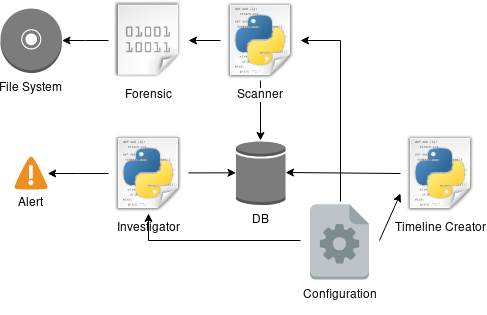
\includegraphics[width=8cm]{../img/Overview_FIDS.png}
  \centering
  \caption{System Architecture}
  \label{fig:systemArchitecture}
\end{figure}

\subsection{Configuration}
\label{sec:Configuration}

The configuration file is provided in \gls{yaml}. \gls{yaml} is a human friendly data serialization language used in many programming languages. Its main advantage over other languages for configuration files is the readability and the ease to extend already existing configuration files. There were more reasons why \gls{yaml} is used documented in section \ref{sec:decisions:config:language}.

\subsubsection{Database Configuration}

The configuration consists of three parts. The first part is the database configuration. Options are to either use the system with a \gls{sqlite} database file, which is the most simple solution, or to use it with a \gls{postgres} database server. For the sqlite configuration only the filename is required as seen in listing \ref{lst:cfg:sqlite}. For a postgres server there needs to be more configuration. The host and port need to be provided, as well as the database, the user and a password as evident in listing \ref{lst:cfg:postgres}. This configuration defines where the data will be sent to and read from in the scanner and investigator parts respectively. As both parts need access to the database this part of the configuration is in a seperate part. It is possible to extend the system to use more \gls{dbms}, it is not part of the scope of this thesis though.

\begin{lstlisting}[language=yaml, numbers=left, caption=SQLite Configuration, label=lst:cfg:sqlite]
sqlite:
	filename: fids_db3.db
\end{lstlisting}


\begin{lstlisting}[language=yaml, numbers=left, caption=Postgres Configuration, label=lst:cfg:postgres]
sqlite:
	filename: fids_db3.db
\end{lstlisting}

\subsubsection{Scanner Configuration}

The second part of the configuration is the part that defines the scanner. An example config can be seen in \ref{lst:cfg:scanner} It consists of one main key which is named scan. If this config entry is missing, the scanner part of the \gls{hids} will not be executed by default. Then it contains the following subkeys:

\begin{itemize}
	\item		\textbf{image\_path} Path to the \gls{fs} that is used for the scan.
	\item		\textbf{scan\_paths} List of paths to scan. Paths will be scanned recursively. "/" will thus scan all the paths.
	\item		\textbf{ignore\_paths} Paths that should not be scanned. Can be a subdirectory of any path in scan paths. The recursion will stop at this path and not continue downwards. Practical if certain directories are not interesting for intrusion detection.
\end{itemize}

\begin{lstlisting}[language=yaml, numbers=left, caption=Scanner Configuration, label=lst:cfg:scanner]
scan:
	image_path: /dev/nvme0n1p5
	scan_paths: 
		[
			"/",
			"/nonExisting",
		]
	ignore_paths: 
		[
			"/temp/"
		]
\end{lstlisting}

\subsubsection{Investigator Configuration}

The investigator configuration is simmilar to the scanner configuration in the way that it contains a top level node called detection. If this is missing the investigator part will not start. As can be seen in listing \ref{lst:cfg:investigator} it has the following subkeys:

\begin{itemize}
	\item \textbf{relevant\_paths} This configuration specifies which paths need to be evaluated for the following changes. 
	\item \textbf{filename\_regex} This configuration specifies the regex which the files need to confirm to.  
	\item \textbf{same\_config} This configuration specifies whether a changed config should result in an alert. Defaults to True.
	\item \textbf{greater} This configuration specifies all the attributes that need to be equal or greater than for the previous run.
	\item \textbf{equal} Simmilar to greater, this configuration specifies all the attributes that need to be equal to the previous run.
\end{itemize}

\begin{lstlisting}[language=yaml, numbers=left, caption=Investigator Configuration, label=lst:cfg:investigator]
detection:
	relevant_paths:[
		"/"
	]
	filename_regex: ''
	greater: [
		"meta_size"
	]
	equal: [
		"meta_creation_time"
	]
	same_config: True
\end{lstlisting}

\subsubsection{Aide Configuration}
\label{sec:aide:config}



\subsection{Database}
\label{sec:Database}

The database is another component that is shared between the scanner and the investigator. As already mentioned, multiple \gls{dbms} can be used in conjunction with this \gls{hids}. In this section I will not focus on the \gls{dbms} used. The database consists of five relations. Firstly, I will explain some reoccuring types, how they are stored and what they represent after that, the relations and then quickly how the different \gls{dbms} can be used. 

Some ideas are not specific to a relation. Most relations contain timestamps and \gls{uuid}. How they are stored can be seen below:

\begin{description}
	\item [Timestamps] To save space, Timestamps are stored as an integer value. This value represents the \gls{unixts}. 
	\item [\gls{uuid}] \gls{id} are stored as \gls{uuid} in their \gls{hex} representation. 
	\item [Enum] \gls{tsk} defines many enums. Most of those enums have an int representation. To save space, this representation is stored in the database. The enums can be viewed in the \gls{tsk} \gls{api} reference. \cite{tsk:file:header}
\end{description}

\subsubsection{FIDS\_RUN}

The run table is relatively simple. It contains a \gls{id} so that each run can be identified. This \gls{id} will be used in the other relations as well to create a link to the run. Besides that it contains a \gls{sha256} hash of the configuration that it was started with. It then contains a start and and end time of this particular run. The table definition is shown in listing \ref{lst:cfg:fids:run}

\begin{lstlisting}[language=sql, numbers=left, caption=Fids Run Table Definition, label=lst:cfg:fids:run]
CREATE TABLE FIDS_RUN(
	id varchar(32), 
	config_hash varchar(64), 
	start_time int, 
	finish_time int, 
	PRIMARY KEY(id)
);
\end{lstlisting}



\subsubsection{FIDS\_ERROR}

With each run there is the possibility of errors. Those errors are stored in this table. It is rather simple as well. Additionally to the run \gls{id} it contains an \gls{id} as well. Next to that it contains a description and a location of where it occured. The table definition is shown in listing \ref{lst:cfg:fids:error}

\begin{lstlisting}[language=sql, numbers=left, caption=Fids Error Table Definition, label=lst:cfg:fids:error]
CREATE TABLE FIDS_ERROR(
	run_id varchar(32), 
	id varchar(32), 
	description text, 
	location varchar(255), 
	PRIMARY KEY(run_id, id)
);
\end{lstlisting}

\subsubsection{FIDS\_FILE}

This table contains most of the information. It again has \gls{id} additional to the \gls{id} of the run. Then it has the path in which the file was located and all the meta information about the file. Most attributes start with meta, while the rest start with name. This is a reference to \gls{tsk} which has multiple structs for meta and name information about each file. I kept the naming of \gls{tsk}, thus more information about each attribute can be found on the \gls{api} reference of \gls{tsk}. \cite{tsk:file:struct} The table definition is shown in listing \ref{lst:cfg:fids:file}

\begin{lstlisting}[language=sql, numbers=left, caption=Fids File Table Definition, label=lst:cfg:fids:file]
CREATE TABLE FIDS_FILE(
	run_id varchar(32),
	id varchar(32),
	path text, 
	meta_addr int,
	meta_access_time int,
	meta_access_time_nano int,
	meta_attr_state int,
	meta_content_len int,
	meta_content_ptr int,
	meta_creation_time int,
	meta_changed_time int,
	meta_creation_time_nano int,
	meta_changed_time_nano int,
	meta_flags int,
	meta_gid int,
	meta_link int,
	meta_mode int,
	meta_modification_time int,
	meta_modification_time_nano int,
	meta_nlink int,
	meta_seq int,
	meta_size int,
	meta_tag int,
	meta_type varchar(255),
	meta_uid int,
	name_flags int,
	name_meta_addr int,
	name_meta_seq int,
	name_name int,
	name_size int,
	name_par_addr int,
	name_par_seq int,
	name_short_name int,
	name_short_name_size int,
	name_tag int,
	name_type varchar(255),
	PRIMARY KEY (run_id, id)
);
\end{lstlisting}

\subsubsection{FIDS\_FILE\_ATTRIBUTE}

In \gls{tsk} each file can contain multiple attributes. Those attributes are stored in this table. It contains the previous \gls{id} and another one for each attribute as each file can have multiple attributes. The attributes contain flags, a name and a type. The flags and the type enums called `TSK\_FS\_ATTR\_FLAG\_ENUM' and `TSK\_FS\_ATTR\_TYPE\_ENUM'. More information available in the \gls{tsk} \gls{api} reference. \cite{tsk:attr:struct,tsk:file:header} The table definition is shown in listing \ref{lst:cfg:fids:file:attr}

\begin{lstlisting}[language=sql, numbers=left, caption=Fids File Attribute Table Definition, label=lst:cfg:fids:file:attr]
CREATE TABLE FIDS_FILE_ATTRIBUTE(
	run_id varchar(32),
	file_id varchar(32),
	id varchar(32),
	flags int,
	tsk_id int,
	name varchar(255),
	name_size int,
	at_type varchar(255), 
	PRIMARY KEY (run_id, file_id, id)
);
\end{lstlisting}

\subsubsection{FIDS\_FILE\_ATTRIBUTE\_RUN}

Attributes can contain multiple data runs. Those data runs are represented in this relation. It contains all the \gls{id} from the attributes and an additional for the run. It then has a block address and a lenght. More information can again be found in the \gls{tsk} \gls{api} reference. \cite{tsk:attr:run:struct} The table definition is shown in listing \ref{lst:cfg:fids:file:attr:run}

\begin{lstlisting}[language=sql, numbers=left, caption=Fids File Attribute Run Table Definition, label=lst:cfg:fids:file:attr:run]
CREATE TABLE FIDS_FILE_ATTRIBUTE_RUN(
	run_id varchar(32),
	file_id varchar(32),
	attribute_id varchar(32), 
	id varchar(32), 
	block_addr int, 
	length int, 
	PRIMARY KEY(run_id, file_id, attribute_id, id) 
);
\end{lstlisting}

\subsection{Shared}

There are other shared components. Mainly the model of the system. It contains of multiple classes for the types. There is one class for each relation. They can parse \gls{tsk} objects and they can parse database rows. This way both the scanner and the investigator can work with the same classes. Except for parsing they don't have any functionality.


\section{Application Flow}
\label{sec:flow}

The main application flow consists of first reading the config file. If no config file path is passed the default path is used. It then starts the scanner if a scan configuration is found. After the scanner is completed it starts the investigator if the detection config is found. It works if any of the two configs are found. If none is found then the system will simply do nothing. 


\subsection{Scanner}
\label{sec:Scanner}

The scanner component is the first specific component. It is executed when the system is run and a scan config is available. It is responsible for getting all the information from the \gls{fs} for the configured paths. It has multiple stages.

\begin{enumerate}
	\item Initialization
	\item Scan
	\item Error Logging
	\item Storing
	\item Error Logging
	\item Finalizing
\end{enumerate}

In the initialization phase the scanner creates a run object. This object is already saved to the database. This way user know just by looking at the database if there are any runs still running. This also creates a first opportunity to look for inconsistencies. If there are a lot of started runs, something suspicious might be going on. It also creates the hash of the configuration and already saves it to the database.

The scan phase has more steps to it. First it creates the \gls{pytsk} object called `img\_info'. This is done by passing the path to the disk image to \gls{pytsk}. Then the actually important `fs\_info' object is created by passing the img info object. This way we have access to the \gls{fs}. The scan actually starts by calling `open\_directory\_rec' for each scan path. This function keeps track of all diretories it already traversed into as to avoid circular loops and unnecessary steps. Then it checks if the path is in the ignored paths. It then iterates over all objects in the directory. 

For all entries it checks if it is a valid entry with the required attributes to continue. Afterwards it checks if it is a directory. For all the directories the function first checks if the directory has already been visited and if not it calls itself with the new directory as the parameter. If the entry is a file, it is parsed into a python object and then stored into a local list of found files. Any errors that occur are saved by creating an error object that is stored into a list of errors.

In the error logging phase all errors that have occured in the scan process are stored in the database. This is done by iterating over all the errors and saving them one by one. The database is then commited and even if the files can't be saved for some reason, the errors will be persisted.

After the first error logging phase is the file saving phase. Here the files are saved again by iterating over them and saving one by one. Should any additional error occur while saving the files, they are again added to a list of errors. 

There is a second error logging phase. In this phase the errors that occured while saving the files get stored into the database. The functionality is the same as for the first error logging phase.

In the finalizing phase the run object gets updated and the endtime added. It is then also updated on the database. At this point the scanner is finished. It has written all the files from the \gls{fs} to the database. Also all errors that occured during this process are logged. The run object on the database will have a valid start and end timestamp. 


\subsection{Investigator}
\label{sec:Investigator}

TODO: finish investigator logic first. Could document current logic, but is not useful as it is not fast enough. 

\section{Security}
\label{sec:Security}

A \gls{hids} is a system that tries to improve the security of a host by detecting intrusions. Thus, it is extremely important to evaluate the security of such a system. This is the goal of this section. First, I will show some limitations of the produced system. It has some downsides and it is important to look at them. After that I will loook at some risk associated with running the \gls{hids}. Those risks might be associated with all competitors. Then I will give some attack scenarios. Those will include some scenarios where the proposed \gls{hids} is better suited than previous \gls{hids}, but also some that specifically attack the limitations and risks. Lastly, I will dive into how to circumvent those attack scenarios. Some might be defeated if we change some small things, some will need more work.

\subsection{Limitations}
\label{sec:Limitations}

There are multiple limitations that I will list below. I will reference those in the attack scenarios and mittigations. I will also list how easily they can be exploited and how easy it is to detect those limitations.

\subsubsection{Changing Attributes}
\label{sec:limitation:chattr}
As already mentioned multiple times, the proposed system doesn't use \glspl{hash} for detection of intrusions. This is a big issue as it means that changed files might not be found. Attributes can be changed which could lead this implementation to miss an intrusion.  \cite{chaning:times, changing:attributes}

It is rather easy to change the \gls{fs} attributes. However, it is not trivial to change all of them. Some will leave traces and for some attributes root access is needed. Additionally the attacker would first need remember the times which would be correct such that he can correctly reset the times. This can be quite challenging. However, it is likely that the attacker will not change all attributes or that he sets them incorrectly, such that the system can still discover the changes. Some changes to the attributes will leave other traces, such as kernel level logs. Those can be evaluated to find this kind of intrusion.

\subsubsection{Non file based intrusion}
\label{sec:limitation:nonFileBased}
Another limitation are intrusions that are not file based, which are getting more popular even as \gls{apt}. Many of the biggest threats for web applications according to \gls{owasp} are not creating any files on the host. \cite{owasp} There are also other attacks which don't need to use files if they can hijack an already started process. Those attacks are not detectable because the system only works on file basis.

Those kind of intrusions are getting more common and as already said, can't be discovered by only checking the \gls{fs}. However, they leave other traces. They often leave logs in the application because for most of the \gls{owasp} top ten, many trial and error is required. For \gls{apt} it is more difficult to find them. They mostly leave traces as well in form of weird network behaviour. Because to achieve persistance they need to redownload the malware after a host has been rebooted.

\subsubsection{Intrusion in non watched location}
\label{sec:limitation:nonWatched}
When the scanner is started it is fed with which paths to scan and which to ignore. If an intrusion injects a file in a place that is not watched, it will not be found. This limitation comes from a faulty configuration.

For non watched locations it is as if the host would not run a \gls{hids}. Maybe the intrusion will at some point write or read something in a watched location, but otherwise the threat can go unnoticed for a long time. To avoid such intrusions it is recommended that at least the scanner part of the \gls{hids} on the whole system. Additionally it is recommended to run the investigator on the whole system as well, but maybe with a lower frequency.

\subsubsection{Preexisting intrusions}
\label{sec:limitation:preexisting}
The system can only detect intrusion by unexpected changes. If it is started on an already running host, it is possible that this host is already infected. This infection can not be seen by the system, as long as the files from the intrusion stay consistent. 

Preexisting intrusions are hard to detect if they don't alter their files. Luckily malware behaves like a normal software project. At some point it will probably change its executable. It might also read or write other files that seem suspicious. Additionally, if the \gls{hids} is deployed with new machines additionally to the already running machines, those are going to detect the intrusion as soon as the already infected hosts try to infect the newly deployed ones.

\subsubsection{Shut down \gls{hids}}
\label{sec:limitation:noscan}
The system relies on the running of the scanner. On a host this would probably be done by creating a scheduled task. If this can be disabled, then the scanner will no longer run and no further intrusions will be detected. Additionally the investigator could also be stopped. This would lead to the same issue.

Should the scanner be shut down then the investigator will no longer find any intrusions. This can be detected if the database is checked on new entries from another source. This is easiest done when an external database is used or when the sqlite file is copied from the host to an external machine at some points. Also, if logs are configured to be written after each execution, it can be suspicious if those entries are missing or are showing to be evaluating the same runs over and over again. 

This limitation is not highly likely, because the intruder first needs to get administrative access to the host to be able to shut down the \gls{hids}. This is not always easy to achieve and once the attacker has administrative access he can do whatever he want on the system. 

\subsection{Risks}
\label{sec:risk}

Aside from the limitations there are some risks with running this system. As with the limitations, I will give some comment to each risk and talk about how to evaluate them.

\subsubsection{Running unknown code}
\label{sec:risk:unknowncode}

As for any program, it is always a risk associated to execute code that was downloaded from the internet. It is possible that it was modified or that it is exploitable. However, this is an \gls{opensource} program. This makes it easier to evaluate the code. The same would need to be done for all the dependencies, more specifically for \gls{pytsk} and \gls{tsk}. This is possible but requires a lot of work. However, the \gls{opensource} community is generally well trusted, which might be enough. To protect from alterations to the tool that was downloaded, hashes can be validated. Additionally, the system behaves very straightforward. It will scan the file system and then write to a database. It will then read from the database and create alerts. This functionality can be monitored. Should the system do something else it might either have a bug or is being abused.

\subsubsection{File access}
\label{sec:risk:file}

Any \gls{hids} that operates on file basis needs access to the files. Depending on the data that is stored on the host this might be a cause for concern. The system has full access on any of those files. This can not be circumvented. What can be done is using only the scanner on this system. Let it write either to a centrally managed database or a sqlite file. Then let the investigator run on the data from another host. This way the system can be monitored to make sure it doesn't open any other communication.

\subsubsection{Root access}
\label{sec:risk:root}

The system needs access to the disk image which is mounted. To gain access to that it needs to run with administration privileges. With those permissions the system could theoreically do anything on the host. The best way would be to limit the amount of time that it is executing with those privileges. To do that the scanner and the investigator can be executed in different processes where only the scanner has administrative access. The investigator only needs to read the database and send alerts, for neither it needs administrative privileges.

\subsection{Attack Scenarios}
\label{sec:attack_scenarios}

In this section I describe several attack scenarios. I will only explain what the intruder does and how he does it. I might give some description of the host and which processes are running. I will also list which limitations or which risks the attacker uses. In section \ref{sec:mittigations} I explain how those attacks can be avoided or detected and what is needed for the detection. Finally in the discussion I give a short summary on how my system stands against other systems like Aide. 

\subsubsection{Classic Intrusion with persistance}
\label{sec:attack:classic}

The classic way to gain a foothold on a host is to write a file on the \gls{fs}. This file is then executed remotely and the host is compromised. How exactly the attacker was able to upload a file is not relevant for this scenario. The attacker will not do anything special with the file and leave it where it lands. He does not change any attributes or uses any other tactic to hide.

This attack actually exploits none of the risks and limitations as this is the basic kind of attack that the system is made to find. 

\subsubsection{Intrusion with persistance, attacker changes all metadata}
\label{sec:attack:changeattr}

The attacker is able to change a file or create a file on the host and then resets the attribes in such a way that the system can't find anything wrong.

Risks and Limitations:
\begin{itemize}
	\item \nameref{sec:limitation:chattr}
	\item \nameref{sec:limitation:nonWatched}
\end{itemize}

\subsubsection{Intrusion without persistance to use as intermediate host}
\label{sec:attack:nopersistanceintermediatehost}

The attacker is able to exploit a running process. He uses the host to gain access to other machines in the network and does not read or write anything from or to the host. 

Risks and Limitations:
\begin{itemize}
	\item \nameref{sec:limitation:nonFileBased}
\end{itemize}

\subsubsection{Intrusion without persistance to exfiltrate data}
\label{sec:attack:nopersistanceexfiltration}

As in scenario named `\nameref{sec:attack:nopersistanceintermediatehost}' the attacker gains access through an exploit of an already running process. However, in this scenario he does read files of interest, for instance private keys for encryption. 

Risks and Limitations:
\begin{itemize}
	\item Partially: \nameref{sec:limitation:nonFileBased}
\end{itemize}

\subsubsection{Intrusion without persistance but as apt}
\label{sec:attack:nopersistanceapt}

This scenario is simmilar as the previous two. Here the attacker is again able to exploit a process that is already running. He then goes on to use this process to do things that are uncharacteristic for this process. He does neither read nor write files from the host. His goal is to stay hidden for as long as possible. Additionally he wants to reinfect the host whenever the process is restarted.

Risks and Limitations:
\begin{itemize}
	\item \nameref{sec:limitation:nonFileBased}
\end{itemize}

\subsubsection{Attacker exploits \gls{hids} to gain administrative privileges}
\label{sec:attack:exploitforroot}

Differently from before, this time the attacker somehow can exploit the \gls{hids} to gain administrative privileges. The most likely way is to give it a different configuration or change the code that is already running on the system. It needs to be either because the scanner subsystem does not have any additional entrypoints.

Risks and Limitations:
\begin{itemize}
	\item \nameref{sec:limitation:nonFileBased}
	\item \nameref{sec:risk:root}
	\item \nameref{sec:risk:unknowncode}
\end{itemize}

\subsubsection{Attacker changes the code maliciously}
\label{sec:attack:codechange}

The attacker is able to change the code that the user downloads. He injects his own malicious code in the version that was downloaded. It is then executed ant the attacker is able to take over the host.

Risks and Limitations:
\begin{itemize}
	\item \nameref{sec:limitation:preexisting}
	\item \nameref{sec:risk:root}
	\item \nameref{sec:risk:unknowncode}
\end{itemize}

\subsection{Attack Mittigations}
\label{sec:mittigations}

To avoid the attacks described in \nameref{sec:attack_scenarios} there are multiple things one can do. First I give some information how the specific scenarios can be detected if possible. Then there are some general recommendations on what can be done to increase the security of the system or of the host.

\subsubsection{Classic Intrusion with persistance}
\label{sec:defense:classic}

This attack scenario is actually the easiest. It will be detected if the system is configured correctly. Compared to other \gls{hids}, this kind of attack will be found faster, because the system can be run more often. 

\subsubsection{Intrusion with persistance, attacker changes all metadata}
\label{sec:defense:changeattr}

This kind of attack can only be found, if the attacker takes longer than the system has to scan. It is possible that the \gls{hids} discovers it while the attacker has not yet changed all the attributes. Additionally, it is possible that the attacker did not change all the relevant attributes. In both cases the system will find the intrusion and alert it. Should the attacker be fast enough the system will not find the changed file. Then it depends on how well the attacker hides. If he does not do anything on the \gls{fs}, it is possible that this kind of intrusion will go unnoticed for a long time by the \gls{hids}. 

Here a \gls{nids} or a different \gls{hids} comes into play. The host can be configured in such a way that there is a different \gls{hids} running that only runs on a part of the \gls{fs} that has more exposure. A \gls{nids} can also detect this kind of intrusion, because the attacker will need to communicate to or from the compromised host at some point. 

\subsubsection{Intrusion without persistance to use as intermediate host}
\label{sec:defense:nopersistanceintermediatehost}

This type of attack can not be detected by any \gls{hids} that only works on file basis. Here again a \gls{nids} can help. Most likely the attacker wants to gain access to other hosts in the network. When there is a \gls{nids} installed, it should be able to detect this traffic and alert them. Another way would be to deploy an additional \gls{hids} that does not work on file basis, but checks network information. This way it would find the intrusion and can alert it.

\subsubsection{Intrusion without persistance to exfiltrate data}
\label{sec:defense:nopersistanceexfiltration}

This type of attack is again very visible for a \gls{nids}. Large amounts of data will be transfered in a way, that might not be usual. This can result in alerts from a \gls{nids}. Here the proposed system might be able to alert the attack as well. As the attacker reads the data, it changes the modified timestamp. If the attacker does not reset this timestamp, the system will be able to alert the change. 

\subsubsection{Intrusion without persistance but as apt}
\label{sec:defense:nopersistanceapt}

This type of intrusion is again not possible to detect by a \gls{hids} that works on file basis, except the attacker reads files. Here again a \gls{nids} is needed which will be able to detect it, because after the infected process is restarted, another host will reinfect it. This is the kind of traffic a \gls{nids} should be able to detect.

\subsubsection{Attacker exploits \gls{hids} to gain administrative privileges}
\label{sec:defense:exploitforroot}

For the system, this attack is probably not detectable, because the attacker changes the system itself. The best way to protect against that is to closely monitor what it does. The scanner part should only be allowed to read data from the disk image and write it to the specified data. To protect further, the investigator should be executed seperately without admin privileges. This way the attack surface is smaller. The only thing that can be used to generate an exploit would be the scanner config. Another way to notice the change might be the changed configuration which might already have been saved to the database. This way one might notice that something is wrong.

\subsubsection{Attacker changes the code maliciously}
\label{sec:defense:codechange}

This attack is not detectable from the system again, because firstly, the system itself was changed and behaves abnoramally. And secondly, because when the system was executed, the intrusion already happened. To protect from this form of attack, the system administrator should check the hash of the \gls{hids}. Additionally, he should verify the \gls{pgp} key. This way an administrator can make sure that the package which is installed has not been altered. Further, the source code can be checked and compiled by the system administrator himself. This would take more work but the possibility for malicious inclusions are fewer. 

\subsection{General defense}
\label{sec:defense:general}

Generally it makes sense to use a \gls{nids} in conjunction with any \gls{hids}. Some intrusions are easier to detect on the host level and others on a network level. Both make sense so both should be used. Additionally, it makes sense to use an additional \gls{hids} which is specialized in detecting intrusions on process or network activity level. This way the host is monitored fully and intrusions can be even better detected. 

For the system specifically, it makes sense to run the scanner and the investigator seperately. To gain the most security, the scanner should run on the system and write the output to a \gls{dbms} which is outside the host with a user that can only append to most tables and additionally update the endtime column of the fids run relation. The investigator should then be started on a seperate host that only validates intrusions. This way the attack surface is as small as possible. 

\chapter{Discussion}
\label{sec:Discussion}

The designed and implemented \gls{hids} works differently than previous \gls{hids}. Many will argue that because it does not generate \glspl{hash} it is insecure. I argue against that, because finding intrusions always takes risks. If a conventional \gls{hids} finds more intrusions but takes a long time to scan the whole system, it is not useful. Finding an intrusion days or even weeks after it happened might not be interesting. The attacker then has a long time to either hide, move on or extract all the information he is interested in. Finding intrusions in a timely fashion is very important and this is where my implementation shines. Additionally, even if it didn't find the intrusion, the database can be very helpful for forensic investigators to find out what the attacker did. This might help finding similar attacks in the future by adapting the configuration or by chaning other components. The argument this system makes is not even to be the one and only. In its current form this does not make sense. I hevily advise people to use a \gls{nids} or a \gls{hids} with other focusses. I also advise people to use a \gls{hids} on file basis which uses \glspl{hash} for highly critical parts of the system. However, if only a hash based \gls{hids} is used, then many attacks will be found to late, or not at all. Another benefit that this implementation has is that it runs on any system. \gls{tsk} runs on Linux, OsX and Windows, so does python. By using those components, this system should work on any of those systems as well.

During my work I realized the system and I tested it with modified data. However, the system has not yet been used in a productive environment and has not yet detected an intrusion. This means that it can not be said without doubt if it would work. The main reason why it has not been tested is that the time ran out. Besides that there were ethical and judical conserns of creating a host that is easily exploitable just so that it can be attacked. This would lead to criminals gaining access to a host to do their work which is not in my interest. Even if my system would find their intrusions, it is still possible that they can abuse the host for some time. Additionally, it is possible that they would use an attack which my system can not detect. This would mean that they have access to the host for a prolonged time. The system would needs to be tested in a live environment where attacks naturally happen. Sadly, I did not have access to such a system. 

\section{Future Work}
\label{sec:future:work}

It would make sense to extend this \gls{hids} to extend past the \gls{fs}. It would be great if the scanner can also scan the processes and network connections. Not only would this data be important to finding intrusions by the system, but it could also give investigators much more information. Information which they are currently mostly missing.

The system should also be extensively tested. For this it needs to run for a prolonged time in a productive system. The output and the found intrusions would then need to be compared to other system to gain important information about how fast and how many intrusions are found using this system. 

One other path that could be improved on would be the investigator. Currently it operates only on a configuration which someone must write. It would be great to autonomously analyse the scanner output and find anomalies on them. This could be done if a lot of data has already been collected on many different types of hosts. The types could then be grouped and an algorithm could detect similar patterns to find simmilar intrusions. 

Generally, the field of finding intrusions has a lot of opportunities for research. This system can be one part of an extensive system that checks for intrusions. Especially since disk sizes and data usage is still growing it is important to have such a system that can find intrusions fast.

\chapter{Conclusion}
\label{sec:Conclusion}

In this thesis the goal was to create a \gls{hids} which finds intrusions in big \gls{fs} fast and helps with forensic investigation. Such a system was built. I am using \gls{tsk} to only check \gls{fs} \gls{metadata} to find intrusions. This way the system is extremely fast compared to systems that use \glspl{hash}. My system thus takes a risk based approach to finding intrusions. It will not find them as reliably as other systems, but it will find them faster. 


\chapter{Journal}

\chapter{Implementation Details}

\section{Decisions}
\label{sec:decisions}

\subsection{Programming Language}
\label{sec:decisions:language}

\subsection{Language for Configuration File}
\label{sec:decisions:config:language}


\chapter{User Documentation}

\chapter{Project Management}

\section{Goal}
\label{apdx-sec:goal}
Before the start of the project the following main goal was defined:

Building of an \gls{hids} that detects unauthorized or unusual behaviour on the file system. Compared to traditional \gls{hids} file system integrity checking, it should scale with a lot of data and have the possibility to be used for investigation (retain historic data) built in from the start.

\subsection{Sub goals}

From this primary goal, the following sub goals were defined. 

\subsubsection{Scanning}
The system is capable of scanning the file system for certain properties. The search is done by leveraging the sleuthkit tools. Thus the system is capable of interpreting the results from sleuthkit. It will further analyze them and decide on what to do with the results. Especially importance is given to the finding of differences.

\subsubsection{Recording}
The system records all findings. Including new, changed and deleted files in comparison to an earlier point in time. This recording enables the use of investigation as the evolution of the data can be viewed at any time. This data can also be used for machine learning algorithms to detect anomalies that are out of the scope of this thesis. 

\subsubsection{Evaluation}
The system is capable of evaluating the results by applying predefined rules. Those rules can be adjusted by configuring the system.

It is thinkable that the system analyzes the recordings and makes decisions based on the historical behavior of the specific host and behavior from different similar hosts. This approach is not part of this thesis as it requires much historical data that is not present at the time of this thesis. 

\subsubsection{Alerting}
The system is capable of being run continuously. This capability enables it to find anomalies automatically. The system can report those anomalies by creating alerts. It allows configuration of these alerts.

\subsubsection{Scaling}
The run of the system on a big file system completes in an appropriate amount of time. This speed allows the finding of anomalies that appeared recently. Additionally, it allows the storing of more states of the system which results in a her probability of capturing short-lived anomalies for future investigations. 

\section{Workpackages}

From those goals the workpackages in table \ref{tab:workpackages} were defined. For a better overview they are assigned to categories. The categories are Architecture, Implementation, Validation and Administrative. Architecture is about defining how the system will look like and how it should work. Implementation is the effective implementation work for getting the system to run, this includes configuration and coding. Validation is about testing of the system. Administrative is everything that deals with project management and other workpackages that don't directly influence the system but need to be done.

The ID is a combination of the first letter of the category and a unique index. Administrative is shortened to D due to the conflict with Architecture.

The priority is a value of high, medium and low. 

The workpackages are chrononically ordered. Meaning they should be worked on in approximately the order that they are given. 

\begin{table}[h!]
  \begin{center}
    \caption{Workpackages}
    \label{tab:workpackages}
    \begin{tabular}{c|l|c|l}
      \textbf{ID} & \textbf{Short description} & \textbf{Prio} & \textbf{Category} \\
      \hline
      D00 & Setting up \LaTeX -document & h & Administrative \\
      D01 & Define workpackages and set deadlines & h & Administrative \\
			A00 & Research other \gls{hids} and the sleuthkit tools & h & Architecture \\
			A01 & Decide on a Programming Language & h & Architecture \\
			I00 & Setup the developer environment & h & Implementation \\
			I01 & Add the ability to scan the whole system using sleuthkit & h & Implementation \\
			A02 & Decide which database connectors should be used & h & Architecture \\
			I02 & Add one database connector & h & Implementation \\
			I03 & Implement a recording functionality & h & Implementation \\
			A03 & Decide how the rules should be defined & h & Architecture \\
			I04 & Add template rules and ability to parse them & h & Implementation \\
			I05 & Add functionality to parse output according to rules & h & Implementation \\
			V00 & Verify that the system runs on a big file system & h & Validation \\
			I06 & Add functionality of repeated scans & m & Implementation \\
			A04 & Define which alerting methods make sense & m & Architecture \\ 
			I07 & Add alerting functionality using one method & m & Implementation \\
			V01 & Verify the functionality of the software by changing the system & h & Validation \\
			V02 & Verify the functionality of the software by running it on an infected system & m & Validation \\
			V03 & Verify the alerting of the software by running it on an infectable system & m & Validation \\
			I08 & Add multiple database connectors to different systems & m & Implementation \\
			I09 & Add multiple alerting methods & m & Implementation \\
			A05 & Define how to protect system and configuration from tampering & l & Architecture \\
			I10 & Implement software hardening & l & Implementation \\
			D02 & Finish user documentation & m & Administrative \\
			D03 & Finish project documentation & h & Administrative \\ 
			D04 & Create project presentation & h & Administrative \\
			D05 & Create project poster & m & Administrative \\
			D06 & Create project video & l & Administrative \\
    \end{tabular}
  \end{center}
\end{table}

\section{Planning}

For the planning of this project the following milestones were created. Each coveres multiple workpackages. The mapping can be seen in table \ref{tab:milestones}. The milestones can also be seen in figure \ref{apdx-fig:milestones}. There they are displayed with an assumed and actual finish date.



\begin{table}[h!]
  \begin{center}
    \caption{Milestones}
    \label{tab:milestones}
    \begin{tabular}{c|l|c|l}
      \textbf{ID} & \textbf{Short description} & \textbf{Workpackages} \\
      \hline
			00 & Setup & D00, D01, A00, A01, I00 \\
			01 & Initial functionality & A02, I01, I02, I03 \\
			02 & Rules & A03, I04, I05, V00 \\
			03 & Alerting & A04, I06, I07 \\
			04 & Exhaustive testing & V01, V02, V03 \\
			05 & Usability & I08, I09, D02 \\
			06 & Software Hardening & A05, I10 \\
			07 & Presentation & D02, D03, D04, D05, D06 \\
    \end{tabular}
  \end{center}
\end{table}


\begin{figure}[H]
	\begin{ganttchart}[
		hgrid,
		vgrid,
		x unit=7mm,
		y unit chart=10mm,
		milestone label font = \footnotesize
	]{1}{17}
	\gantttitle{2019}{17}\\
	\gantttitlelist{1,...,17}{1}\\
	
	\ganttplannedmilestone{Setup}{4}
	\ganttactualmilestone{}{0}\\
	\ganttplannedmilestone{Initial functionality}{5}
	\ganttactualmilestone{}{0}\\
	\ganttplannedmilestone{Rules}{7}
	\ganttactualmilestone{}{0}\\
	\ganttplannedmilestone{Alerting}{8}
	\ganttactualmilestone{}{0}\\
	\ganttplannedmilestone{Exhaustive testing}{10}
	\ganttactualmilestone{}{0}\\
	\ganttplannedmilestone{Usability}{13}
	\ganttactualmilestone{}{0}\\
	\ganttplannedmilestone{Software Hardening}{15}
	\ganttactualmilestone{}{0}\\
	\ganttplannedmilestone{Presentation}{17}
	\ganttactualmilestone{}{17}
	\end{ganttchart}
	\caption{Milestones}
	\label{apdx-fig:milestones}
	\end{figure}

\section{Meetings}

\subsection{Template}

Hi Bruce,

Next Meeting:

Discussions:

Next Steps:

Julian


\newpage



\clearpage


\printglossaries

\clearpage

%% Print the bibibliography and add the section to the table of content
\printbibliography[heading=bibintoc]

%% Print the bibibliography and add the section to the table of content

\end{document}
